\introduction  %% \introduction[modified heading if necessary]


\begin{figure}
\centering
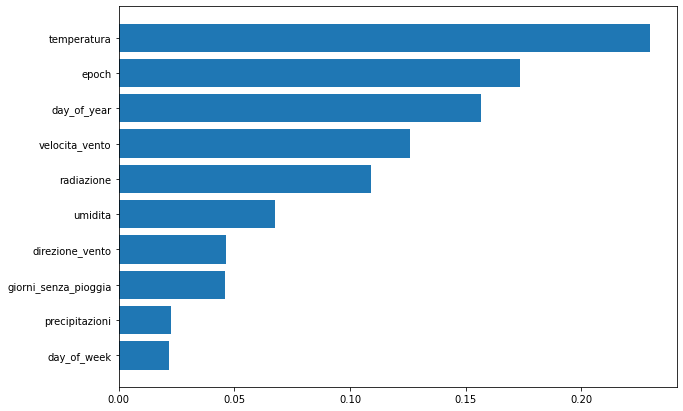
\includegraphics[width=0.75\textwidth]{intro_importanza_totale}
\caption{Media delle importanze delle variabili predittrici nei modelli generati durante le nostre analisi}
\label{fig:importanza_tot}
\end{figure}

\todo{contesto aria lombardia}

\todo{trend **storici**, mancano i grafici}

\todo{riprendere da capitolo 3 della tesi, ma solo le parti che ancora non includono le relazioni fra le varie variabili}

\todo{contestare la percezione (articolo rapporto EU)}

\todo{rete misurazione ARPA}

\todo{scopo: scorporare grande variazione causata dal meteo per evidenziare cambiamenti nel quadro emissivo}

\todo{ulteriore: periodo COVID e influenza del traffico sull'inquinamento, areac}

\todo{carrellata delle variabili che sono state prese in considerazione}



\todo{tradurre e sintetizzare}


L'inquinamento atmosferico è un tema che viene spesso discusso e dibattuto, visto che respirare un'aria pulita è considerato un requisito basilare per la buona salute umana. Da anni il WHO \cite{world2006air} si occupa di studiare i potenziali effetti dell'inquinamento sulla salute umana, cercando di stimare che tipo di impatto possa avere un'esposizione prolungata ad alte concentrazioni.  

Chiaramente non è facile riuscire a stabilire con certezza il collegamento tra causa (esposizione agli inquinanti) ed effetto (malattie e morte) poiché spesso i danni si manifestano solo a seguito di ripetute e prolungate esposizioni, così come non è facile riuscire a stabilire con certezza che una morte sia stata causata esplicitamente dall'inquinamento atmosferico.  

L'inquinamento atmosferico è un fenomeno molto complicato da analizzare, poiché sia per quanto riguarda la produzione e l'emissione in atmosfera che per la dispersione entrano in gioco molti fenomeni e fattori, che hanno scale spaziali molto differenti e che è difficile riuscire ad analizzare correttamente.  

Se in alcune zone del mondo, soprattutto quelle dei paesi in forte via di sviluppo come il sud-est asiatico o l'India, l'inquinamento rappresenta ancora un problema molto grave causato dall'aumento del fabbisogno energetico che è stato soddisfatto incrementando l'uso di combustibili fossili, in Europa (come in altre parti del mondo) negli ultimi 25 anni si è registrato un disaccoppiamento tra la crescita economica e le emissioni dei principali inquinanti, causato da un maggiore impegno nel loro contenimento da parte dei governi, che hanno imposto limitazioni e misure sempre più stringenti \cite{cattani2014analisi}.

È quindi normale che sia la comunità scientifica che le autorità incaricate di decidere le misure di contenimento da mettere in campo siano interessate a capire quale sia il reale andamento delle concentrazioni di inquinanti, cercando di identificare quali possano essere i metodi più efficaci e quanto le variazioni registrate siano attribuibili specificatamente ai cambiamenti delle emissioni umane rispetto agli effetti di altri fattori come il clima che possono avere un'influenza molto maggiore sulle concentrazioni registrate \cite{porter2001ozone}.  

Quasi tutti gli inquinanti di maggior interesse, come gli ossidi di azoto, il biossido di zolfo, il monossido di carbonio, il particolato e l'ozono sono infatti caratterizzati da una forte variabilità stagionale che, per esempio, non ci permette di confrontare valori registrati durante la stagione estiva con quelli invernali, così come l'azione di agenti atmosferici come il vento e la pioggia possono portare ad abbattimenti delle concentrazioni. Nella pianura padana, per esempio, è infatti frequente assistere, specialmente nei mesi invernali che sono già quelli più critici per le concentrazioni di molti inquinanti, a lunghi periodi senza precipitazioni che portano a grossi aumenti delle concentrazioni, che però vengono rapidamente abbattute all'arrivo della pioggia.   

Per poter quindi trarre delle conclusioni oggettive sullo stato della qualità dell'aria, riuscendo ad identificare le cause delle variazioni che si registrano e quindi a capire anche l'efficacia delle misure prese, nel corso degli ultimi anni molti studi si sono avvalsi di diverse tecniche statistiche/probabilistiche per poter fare un'analisi oggettiva sugli andamenti dell'inquinamento atmosferico \cite{cattani2014analisi,rao1994detecting,libiseller2005meteorological,pbl2010trends}.
%\todo{atrent: potrebbe valer la pena riportare alcuni concetti dai paper citati?
%marco: vedi frase sotto}
In tutti gli studi si è evidenziato come considerare anche la meteorologia durante l'analisi delle concentrazioni degli inquinanti, cercando di eliminarne l'influenza, sia fondamentale per poter capire come dei cambiamenti nel quadro emissivo vengano riflessi sulle concentrazioni misurate. Questo poi ci permette di poter fare delle analisi oggettive e quantitative più precise sui trend delle serie storiche, qualsiasi sia la località considerata, visto che i metodi utilizzati sono facilmente generalizzabili allo scenario che si vuole considerare in ogni analisi specifica. 

Riuscire ad avere a disposizione tecniche e modelli che ci permettono di analizzare l'andamento delle concentrazioni e ad identificare le cause che possono cambiare questo andamento ci permette di capire quali siano le aree più critiche su cui andare ad intervenire ma ci può anche permettere di identificare gli interventi più efficaci e sui quali conviene investire maggiormente. La crescita economica e l'aumento del fabbisogno energetico rendono quindi fondamentale il controllo delle emissioni, per poter mantenere la qualità dell'aria a livelli non pericolosi per la salute umana e al tempo stesso non bloccare le attività economiche.  

Qualsiasi studio sui trend degli inquinanti, così come qualsiasi conclusione che ne può derivare, non possono quindi non tener conto degli effetti della meteorologia sulle concentrazioni, poiché i risultati che si otterrebbero correrebbero il rischio di non rappresentare il cambiamento nelle emissioni antropiche ma anche una variazione nei fenomeni atmosferici e negli agenti climatici.  

Il nostro obbiettivo è quindi stato quello di ricercare una tecnica per normalizzare i dati sull'inquinamento rispetto alla meteorologia e al clima, ovvero che fosse in grado di eliminare l'influenza degli agenti atmosferici come pioggia, vento e radiazione solare e della stagionalità che porta ad avere condizioni più o meno favorevoli alla dispersione dalle concentrazioni registrate degli inquinanti, in modo da arrivare poi ad avere una serie storica su cui poter fare analisi sull'efficacia delle misure prese nel corso degli anni per il contenimento delle concentrazioni.  

Un metodo comune per riuscire a fare questa ``pulizia''%\todo{atrent: le virgolette si fanno così} 
dei dati si basa sulla creazione di modelli statistici che tramite l'uso di diverse variabili \textit{predittrici}
%\todo{atrent: andrà spiegato bene cosa si intende col termine, qui lo metterei tra virgolette o in corsivo
%marco: predittrici è il nome formale delle variabili nei modelli statistici
%atrent: forse meglio citare/spiegare il termine ``proxy''
%marco: ho aggiunto una nuova frase che credo spieghi abbastanza bene il termine predittrici, non ho citato il termine proxy perchè la definizione statistica non corrisponde con quella di variabile predittrice}
, come le misure meteorologiche su vento, precipitazioni e radiazione solare e variabili temporali legate al giorno dell'anno e alla date, siano capaci di prevedere i valori delle concentrazioni che si sarebbero misurate per un inquinante in base ai valori di ciascuna. Col termine variabile predittrice, infatti, si intende una variabile in grado di spiegare, anche solo parzialmente, cambiamenti nel valore di un'altra variabile, permettendo quindi di fare previsioni su di esso basandosi sul valore della prima. Se i modelli che riusciamo a creare si rivelano abbastanza precisi nell'attività predittoria e in grado di spiegare buona parte della varianza delle concentrazioni allora possiamo usarli con una certa confidenza per eliminare gli effetti della meteorologia dalle concentrazioni di inquinanti.

% nota per me (atrent)
% step 1: trovare predittrici
% step 2: usarle per scorporare effetto

Questo procedimento viene però complicato dal fatto che le dinamiche che portano la meteorologia a modificare le concentrazioni varino molto a seconda della località e che quindi differenti contesti, come ad esempio possono essere una città rispetto ad una località montana o situata a fondo valle, necessitino trattazione specifiche a seconda del caso. Inoltre è chiaro come le variabili meteorologiche tra di loro siano collegate e correlate, cioè che cambiamenti nei valori di una vengano riflessi anche sulle altre, e questo porta all'insorgere di una serie di problemi come la normalità, la multi collinearità e l'indipendenza che rendono la trattazione con diversi metodi molto difficile e complicata \cite{gunst1975regression}. 
%\todo{atrent: spiegare i termini o citare biblio
%marco: aggiunta breve spiegazione più bib
%atrent: ottimo collegamento con introduzione del termine proxy sopra
%marco: non ho introdotto il termine proxy, ma comunque è spiegato cosa si intende quando si dice che i valori di una variabile influenzano quelli di un'altra}

Nel corso degli ultimi tre decenni nel mondo dell'informatica ha preso campo un'area detta \textit{machine learning} (ML)
%\todo{atrent: almeno un ref sul ML, anche un testo ufficiale o simili
%mbelotti: aggiunta ref}
, che fa uso dei computer e della statistica per creare dei modelli predittori che potessero porsi come alternativa ai classici metodi statistici già esistenti \cite{james2013introduction}. Sono quindi state sviluppate tecniche di ML non parametriche, ovvero che non necessitano di fare alcun tipo di assunzione statistica sulle variabili considerate, che, grazie all'uso dei computer per analizzare grosse moli di dati, permettono di arrivare alla creazione di modelli con buone capacità predittive anche senza occuparsi dei problemi che invece caratterizzano gli approcci puramente statistici. Questi ultimi richiedono infatti, prima di poterli applicare, di fare una serie di assunzioni
%\todo{quali?
%marco: specificato alcune delle assunzioni necessarie (le più semplici, perchè alcune richiederebbero una trattazione più specifica dell'argomento per essere introdotte) e aggiunto footnote} 
sui dati considerati, come la linearità della relazione con i valori della variabile da predirre o l'assenza di autocorrelazione\footnote{Per autocorrelazione si intende quel fenomeno per cui i valori di una variabile sono dipendenti dai valori assunti in precedenza dalla stessa}, e su quali siano le relazioni che li legano ed inoltre molte volte anche la matematica necessaria è complicata e richiede particolare attenzione nella trattazione per essere sicuri di ottenere dei risultati attendibili. Gli algoritmi di machine learning, invece, sfruttando la capacità computazionale degli elaboratori, permettono di arrivare ad ottenere dei modelli altrettanto affidabili senza però doversi preoccupare dei diversi aspetti richiesti dalla statistica e che spesso ne limitano l'applicabilità. Inoltre, molte volte, l'obbiettivo dei modelli statistici è quello di inferire il modello dei dati per il caso considerato, ovvero capire come diversi fattori influenzino quantitativamente i valori di una variabile di interesse, mentre nel machine learning l'obbiettivo principale solitamente è quello di essere capaci di fare previsioni precise sui valori di tale variabile in base a quelli dei diversi fattori considerati \cite{breiman2003statistical}. 
%\todo{atrent: spiegare per sommi capi differenza fra i modelli classici e il ML
%marco: aggiunta spiegazione più bib
%atrent: dettagliare un po' meglio
%marco: aggiunte due spiegazioni sui vantaggi del ML rispetto alla statistica, così mi sembra più chiaro}

ARPA Lombardia \footnote{\url{https://www.arpalombardia.it/Pages/ARPA_Home_Page.aspx}}
%\todo{atrent: link
%mbelotti: aggiunta footnote}
possiede, sul territorio regionale, una rete di 85 stazioni fisse che, per mezzo di analizzatori automatici, sono in grado di fornire rilevazioni ad intervalli di tempo regolari, permettendoci di creare quindi un dettagliato catalogo dei valori delle concentrazioni nel corso del tempo. Tutte queste rilevazioni vengono poi rese accessibili liberamente tramite archivi online, per permetterne la libera consultazione da parte di tutti i cittadini.  

Nel nostro studio abbiamo quindi fatto uso di questi dati, unitamente a quelli delle variabili meteorologiche sempre resi disponibili da ARPA Lombardia, per creare tramite l'uso di una tecnica di machine learning chiamata \textit{Random Forest} \cite{breiman2001random}
%\todo{atrent: link/ref
%mbelotti: aggiunta ref}
%\todo{atrent: quando introduci un termine fa messo in corsivo, specie se è inglese}
dei modelli predittivi che ci permettano di arrivare a fare questa normalizzazione delle concentrazioni di inquinanti rispetto alla meteorologia e quindi di analizzare come si sia evoluta la situazione nella nostra regione nel corso degli anni dal 2012 ad oggi, cercando di capire quali siano stati i provvedimenti e gli eventi più efficaci nell'abbattimento delle concentrazioni.  

%Nel capitolo 2 viene introdotto Random Forest e viene mostrato come questa tecnica possa essere utilizzata per eliminare gli effetti della meteorologia e della stagionalità dall'andamento delle concentrazioni.  

%Nel capitolo 3 viene analizzata, utilizzando la tecnica appena discussa, la situazione regionale andando a controllare l'andamento delle serie dei principali inquinanti nei capoluoghi di provincia lombardi.  

%Nel capitolo 4 verranno presentate le analisi svolte sull'influenza del traffico sulle concentrazioni di tre inquinanti: ossidi di azoto, particolato atmosferico (PM10 e PM2.5) e monossido di carbonio.

%Nel capitolo 5 verrà presentata un'analisi del periodo di diffusione dell'epidemia di Covid-19 e di quali siano stati gli effetti del conseguente \textit{lockdown} svoltosi nei mesi di marzo ed aprile sulle concentrazioni.











